\documentclass{beamer}
% \documentclass[notes]{beamer}
% \usetheme{metropolis}
\setbeamertemplate{navigation symbols}{}
\setbeamertemplate{footline}{
  \vspace{-5em}
  \leavevmode%
  \hbox{%
    \hspace*{0.93\paperwidth}%
    \usebeamerfont{footline}\insertframenumber{} / \inserttotalframenumber\hspace*{2ex}%
  }%
  \vskip3pt%
}

\usepackage{tikz}
\usetikzlibrary{shadows,positioning,arrows.meta,fit,shapes.geometric}
\tikzset{
    frame/.style={draw, thick, fill=gray!10, inner sep=0pt},
    row/.style={
        fill=white,
        minimum width=6.6cm,
        minimum height=0.5cm,
        anchor=west,
        font=\ttfamily\small,
        inner xsep=6pt,
        text width=6.3cm,
        align=left,
        append after command={
            \pgfextra{\draw (\tikzlastnode.north west) -- (\tikzlastnode.north east);}
        }
    },
    arrow/.style={->, thick, >=Stealth},
    biarrow/.style={<->, thick, >=Stealth},
    doublearrow/.style={
        ->,
        double,
        line width=0.6pt,
        double distance=1pt,
        >=Stealth,
        thick
    }
}

\usepackage{graphicx} % Required for inserting images
\usepackage{listings} % Required for code snippets
\usepackage{pgfgantt}
\usepackage{stmaryrd}
% These packages are required for list code snippets.
\usepackage{xcolor}
\usepackage{color}
% The following special color definitions are used in the IST Thesis
\definecolor{forestgreen}{RGB}{34,139,34}
\definecolor{orangered}{RGB}{239,134,64}
\definecolor{lightred}{rgb}{1,0.4,0.5}
\definecolor{orange}{rgb}{1,0.45,0.13}
\definecolor{darkblue}{rgb}{0.0,0.0,0.6}
\definecolor{lightblue}{rgb}{0.1,0.57,0.7}
\definecolor{gray}{rgb}{0.4,0.4,0.4}
\definecolor{lightgray}{rgb}{0.95, 0.95, 0.95}
\definecolor{darkgray}{rgb}{0.4, 0.4, 0.4}
\definecolor{editorGray}{rgb}{0.95, 0.95, 0.95}
\definecolor{editorOcher}{rgb}{1, 0.5, 0} % #FF7F00 -> rgb(239, 169, 0)
\definecolor{chaptergrey}{rgb}{0.6,0.6,0.6}
\definecolor{editorGreen}{rgb}{0, 0.5, 0} % #007C00 -> rgb(0, 124, 0)
\definecolor{olive}{rgb}{0.17,0.59,0.20}
\definecolor{brown}{rgb}{0.69,0.31,0.31}
\definecolor{purple}{rgb}{0.38,0.18,0.81}

\newcommand{\changed}[1]{\textcolor{orange}{#1}}

% Symbols for linear logic
\usepackage{cmll}

% For proof trees
\usepackage{bussproofs}

% For multiply counters, which I use for indentation in class environments
\usepackage{calc}

% These are useful!
\providecommand\todo{}
\renewcommand{\todo}[1]{\textcolor{red}{\textbf{#1}}}

% Useful for CLASS snippets
\lstdefinelanguage{CLASS}{
    morekeywords={proc, cut, close, wait, case, of, send, recv, choice, offer, !, ?, print, println, par, let, share, put, take, cell},
    morekeywords=[2]{lint, colint, lbool, colbool, state, usage},
    sensitive=true,
    moredelim=[is][keywordstyle2]{@}{@},
}

% Useful for IR snippets
\lstdefinelanguage{IR}{
    morekeywords={int, bool, string, tag, cont, exponential, cell, type, isValue},
    morecomment=[l]{//},
    sensitive=true,
}

% Color BNF with strings
\lstdefinelanguage{BNF}{
    morekeywords={nl, pid, lab, int, loc, t, t1, t2, c, c1, c2, d, d1, d2, e, prog, proc, entry, block, instr, sl, st, sc, ofs, locb, reqs, flag, expr, tflg, targ, carg, darg, parg, pargs, earg, eargs, case, if, else, str, bool, src, dst},
    sensitive=true,
    morestring=[b]",
    morestring=[b]',
    morecomment=[l]{//},
    morecomment=[s]{/*}{*/},
    moredelim=[is][keywordstyle2]{@}{@},
    alsoletter={:},
    morekeywords=[2]{::=,|,*,+,?},
}

% Slot names
\newcommand{\irs}[1]{\text{\textcolor{lightblue}{#1}}}
\newcommand{\ints}{\irs{int}}
\newcommand{\bools}{\irs{bool}}
\newcommand{\strings}{\irs{string}}
\newcommand{\tags}{\irs{tag}}
\newcommand{\conts}{\irs{cont}}
\newcommand{\exponentials}{\irs{exponential}}
\newcommand{\types}{\irs{type}}
\newcommand{\cells}[1]{\irs{cell}\left[#1\right]}
\newcommand{\vars}[1]{t_{#1}}

% Slot trees
\newcommand{\nilst}{\left[\right]}
\newcommand{\seqst}[1]{\left[#1\right]}
\newcommand{\tagst}[1]{\irs{tag}\left[#1\right]}
\newcommand{\flagsst}[3]{\irs{flags}\left<#1\right>\left[#2\tagsepst{}#3\right]}
\newcommand{\combst}[1]{\text{$<$}#1\text{$>$}}
\newcommand{\tagsepst}{\text{ | }}
\newcommand{\concatst}[2]{#1\oplus#2}

% Slot offset and data location
\newcommand{\offs}[2]{#1\text{$\sim$}#2}
\newcommand{\dataol}[2]{#1.#2}
\newcommand{\datal}[3]{\dataol{#1}{\offs{#2}{#3}}}

% Some notation commands
\newcommand{\sizeof}[1]{\phi\bigl(#1\bigr)}
\newcommand{\dual}[1]{\overline{#1}}
\newcommand{\getinstructions}[3]{\mathcal{I}_P(#1,\,#2,\,#3)}
\newcommand{\getendpoints}[2]{\mathcal{E}(#1,\,#2)}
\newcommand{\getexpression}[2]{\mathcal{I}_E(#1,\,#2)}
\newcommand{\makeblock}[1]{#1 \leftarrow \text{new}_{\text{b}}()}
\newcommand{\makecont}[1]{#1 \leftarrow \text{new}_{\text{c}}()}
\newcommand{\makedata}[2]{#1 \leftarrow \text{new}_{\text{d}}(#2)}
\newcommand{\makedrop}[3]{#1 \leftarrow \text{new}_{\text{e}}(#2,\,#3)}

% Type names
\newcommand{\classt}[1]{\textbf{\textcolor{forestgreen}{#1}}}
\newcommand{\closet}{\classt{close}}
\newcommand{\waitt}{\classt{wait}}
\newcommand{\lintt}{\classt{lint}}
\newcommand{\colintt}{\classt{colint}}
\newcommand{\lboolt}{\classt{lbool}}
\newcommand{\colboolt}{\classt{colbool}}
\newcommand{\lstringt}{\classt{lstring}}
\newcommand{\colstringt}{\classt{colstring}}
\newcommand{\choicet}[1]{\classt{choice of}\,\{#1\}}
\newcommand{\offert}[1]{\classt{offer of}\,\{#1\}}
\newcommand{\labelt}[2]{\classt{$|$\##1}:#2}
\newcommand{\sendt}[2]{\classt{send}\,#1;#2}
\newcommand{\recvt}[2]{\classt{recv}\,#1;#2}
\newcommand{\bangt}[1]{\classt{!}#1}
\newcommand{\whynott}[1]{\classt{?}#1}
\newcommand{\sendtyt}[2]{\classt{sendty}\,#1;#2}
\newcommand{\recvtyt}[2]{\classt{recvty}\,#1;#2}
\newcommand{\statet}[1]{\classt{state}\,#1}
\newcommand{\statelt}[1]{\classt{statel}\,#1}
\newcommand{\usaget}[1]{\classt{usage}\,#1}
\newcommand{\usagelt}[1]{\classt{usagel}\,#1}
\newcommand{\affinet}[1]{\classt{affine}\,#1}
\newcommand{\coaffinet}[1]{\classt{coaffine}\,#1}
\newcommand{\dualt}[1]{\classt{$\sim$}#1}
\newcommand{\rect}[2]{\classt{rec}\ #1;\,#2}
\newcommand{\corect}[2]{\classt{corec}\ #1;\,#2}

% Process names
\newcommand{\classp}[1]{\textbf{\textcolor{darkblue}{#1}}}
\newcommand{\emptyp}{\classp{()}}
\newcommand{\fwdp}{\classp{fwd}}
\newcommand{\cutp}{\classp{cut}}
\newcommand{\parp}{\classp{par}}
\newcommand{\closep}{\classp{close}}
\newcommand{\waitp}{\classp{wait}}
\newcommand{\casep}{\classp{case of}}
\newcommand{\labelp}[1]{\classp{\##1}}
\newcommand{\sendp}{\classp{send}}
\newcommand{\recvp}{\classp{recv}}
\newcommand{\bangp}{\classp{!}}
\newcommand{\whynotp}{\classp{?}}
\newcommand{\callp}{\classp{call}}
\newcommand{\sendtyp}{\classp{sendty}}
\newcommand{\recvtyp}{\classp{recvty}}
\newcommand{\unfoldmup}{\classp{unfold$_\mu$}}
\newcommand{\unfoldnup}{\classp{unfold$_\nu$}}
\newcommand{\corecp}{\classp{corec}}
\newcommand{\sharep}{\classp{share}}
\newcommand{\affinep}{\classp{affine}}
\newcommand{\discardp}{\classp{discard}}
\newcommand{\usep}{\classp{use}}
\newcommand{\cellp}{\classp{cell}}
\newcommand{\releasep}{\classp{release}}
\newcommand{\takep}{\classp{take}}
\newcommand{\putp}{\classp{put}}
\newcommand{\ifp}{\classp{if}}
\newcommand{\elsep}{\classp{else}}
\newcommand{\letp}{\classp{let}}
\newcommand{\scanp}{\classp{scan}}
\newcommand{\printp}{\classp{print}}
\newcommand{\printlnp}{\classp{println}}

% CLASS
\newcommand{\fwdc}[2]{\fwdp\,#1\,#2}
\newcommand{\cutc}[3]{\cutp\,\{#1\,\classp{$|$}#2\classp{$|$}\,#3\}}
\newcommand{\parc}[2]{\parp\,\{#1\,\classp{$||$}\,#2\}}
\newcommand{\emptyc}{\emptyp}
\newcommand{\closec}[1]{\closep\,#1}
\newcommand{\waitc}[1]{\waitp\,#1;}
\newcommand{\choosec}[2]{\classp{\##1}\ #2;}
\newcommand{\casec}[2]{\classp{case}\,#1\,\classp{of}\,\{#2\}}
\newcommand{\labelc}[2]{\classp{$|$}\labelp{#1}:#2}
\newcommand{\sendc}[3]{\sendp\,#1(#2.\,#3);}
\newcommand{\recvc}[2]{\recvp\,#1(#2);}
\newcommand{\bangc}[2]{\bangp\,#1(#2);}
\newcommand{\whynotc}[1]{\whynotp\,#1;}
\newcommand{\callc}[2]{\callp\,#1(#2);}
\newcommand{\sendtyc}[2]{\sendtyp\,#1(#2);}
\newcommand{\recvtyc}[2]{\recvtyp\,#1(#2);}
\newcommand{\unfoldmuc}[1]{\unfoldmup\,#1;}
\newcommand{\unfoldnuc}[1]{\unfoldnup\,#1;}
\newcommand{\corecc}[4]{\corecp\,#1(#2);\,#3\ [#4]}
\newcommand{\typedefc}[2]{\classp{type}\ #1\,\{#2\};;}
\newcommand{\rectypedefc}[2]{\classp{rec}\ \typedefc{#1}{#2}}
\newcommand{\typedefgc}[3]{\classp{type}\ #1(#2)\,\{#3\};;}
\newcommand{\rectypedefgc}[3]{\classp{rec}\ \typedefgc{#1}{#2}{#3}}
\newcommand{\procdefc}[3]{\classp{proc}\ \texttt{#1}(#2)\,\{#3\};;}
\newcommand{\procdefgc}[4]{\classp{proc}\ \texttt{#1}\langle#2\rangle(#3)\,\{#4\};;}
\newcommand{\recprocdefc}[3]{\classp{rec}\ \procdefc{#1}{#2}{#3}}
\newcommand{\recprocdefgc}[4]{\classp{rec}\ \procdefgc{#1}{#2}{#3}{#4}}
\newcommand{\proccallc}[2]{\texttt{#1}(#2)}
\newcommand{\proccallgc}[3]{\texttt{#1}\langle#2\rangle(#3)}
\newcommand{\sharec}[3]{\sharep\,#1\,\{#2\,\classp{$||$}\,#3\}}
\newcommand{\affinec}[1]{\affinep\,#1;}
\newcommand{\discardc}[1]{\discardp\,#1}
\newcommand{\usec}[1]{\usep\,#1;}
\newcommand{\cellc}[3]{\cellp\,#1(#2.\,#3)}
\newcommand{\cellfc}[2]{\cellp\,#1(#2)}
\newcommand{\releasec}[1]{\releasep\,#1}
\newcommand{\takec}[2]{\takep\,#1(#2);}
\newcommand{\putc}[3]{\putp\,#1(#2.\,#3);}
\newcommand{\putfc}[2]{\putp\,#1(#2);}
\newcommand{\ifc}[3]{\ifp\,#1\,\{#2\}\,\elsep\,\{#3\}}
\newcommand{\letc}[2]{\letp\,#1\,#2}
\newcommand{\scanc}[1]{\scanp(#1)}
\newcommand{\printc}[1]{\printp(#1);}
\newcommand{\printlnc}[1]{\printlnp(#1);}

% IR Data Locations
\newcommand{\slotoffset}[2]{#1\text{$\sim$}#2}
\newcommand{\offsetpast}[1]{\text{past}(#1)}
\newcommand{\offsetfuture}[1]{\text{future}(#1)}

% CLASS definitions
\newcommand{\slots}[2]{\mathcal{S}(#1,\,#2)}
\newcommand{\allslots}[2]{\mathcal{S}_T(#1,\,#2)}
\newcommand{\alllocalslots}[2]{\mathcal{S}_L(#1,\,#2)}

% Compiler environment accessors
\newcommand{\polarityof}[2]{#1_{p}(#2)}
\newcommand{\typeidof}[2]{#1_{t}(#2)}
\newcommand{\continuationof}[2]{#1_c(#2)}
\newcommand{\localdataof}[2]{#1_d(#2)}
\newcommand{\offsetof}[2]{#1_o(#2)}
\newcommand{\readlocof}[2]{#1_r(#2)}
\newcommand{\writelocof}[2]{#1_w(#2)}
\newcommand{\advancech}[6]{#1[#2 \overset{#3,#4}{\oplus} (#5,\,#6)]}

% C generator notation
\newcommand{\arch}{\mathcal{T}}
\newcommand{\archlayout}[1]{\arch(\texttt{#1})}
\newcommand{\slotlayout}[2]{\mathcal{L}_{\arch}(#1,\,#2)}
\newcommand{\layoutofvar}[2]{#1(#2)}
\newcommand{\envlayout}{\mathcal{E}}
\newcommand{\envlayouteps}[1]{\envlayout_\text{eps}(#1)}
\newcommand{\envlayoutdrop}[1]{\envlayout_\text{e}(#1)}
\newcommand{\envlayouttype}[2]{\envlayout_\text{ty}(#1, #2)}
\newcommand{\envlayoutcont}[2]{\envlayout_\text{c}(#1, #2)}
\newcommand{\envlayoutlocal}[2]{\envlayout_\text{d}(#1, #2)}

% Optimizer notation
\newcommand{\typeenv}{\theta}
\newcommand{\isvalue}[1]{\mathcal{V}_\typeenv(#1)}
\newcommand{\isdroppable}[1]{\mathcal{D}_\typeenv(#1)}
\newcommand{\iscloneable}[1]{\mathcal{C}_\typeenv(#1)}
\newcommand{\impossible}{\mathbf{impossible}}
\newcommand{\guaranteed}{\mathbf{guaranteed}}
\newcommand{\dependent}[1]{\mathbf{dependent}(#1)}
\newcommand{\depisvalue}[1]{\mathcal{V}(#1)}
\newcommand{\depisdroppable}[1]{\mathcal{D}(#1)}
\newcommand{\depiscloneable}[1]{\mathcal{C}(#1)}

% Session modes
\newcommand{\writemode}{\texttt{write}}
\newcommand{\readmode}{\texttt{read}}

% Indented CLASS environment
\newcounter{indentlevel}
\newlength{\indentstep}
\newenvironment{class}
{
    \begingroup

    \setcounter{indentlevel}{0}

    \setlength{\indentstep}{1.5em}

    \newcommand{\iz}{\addtocounter{indentlevel}{1}}
    \newcommand{\dz}{\addtocounter{indentlevel}{-1}}
    \newcommand{\pz}{\hspace*{\the\indentstep*\value{indentlevel}}}
    \newcommand{\z}{\\&\pz}

    % CLASS
    \let\cuti\cutc
    \renewcommand{\cutc}[3]{\cuti{\iz\z##1\z}{##2}{\z##3\dz\z}}
    \let\pari\parc
    \renewcommand{\parc}[2]{\pari{\iz\z##1\z}{\z##2\dz\z}}
    \let\waiti\waitc
    \renewcommand{\waitc}[1]{\waiti{##1}\z}
    \let\sendi\sendc
    \renewcommand{\sendc}[3]{\sendi{##1}{##2}{##3}\z}
    \let\recvi\recvc
    \renewcommand{\recvc}[2]{\recvi{##1}{##2}\z}
    \let\choosei\choosec
    \renewcommand{\choosec}[2]{\choosei{##1}{##2}\z}
    \let\casei\casec
    \renewcommand{\casec}[2]{\casei{##1}{##2\z}}
    \let\labeli\labelc
    \renewcommand{\labelc}[2]{\iz\z\labeli{##1}{##2}\dz}
    \let\unfoldmui\unfoldmuc
    \renewcommand{\unfoldmuc}[1]{\unfoldmui{##1}\z}
    \let\unfoldnui\unfoldnuc
    \renewcommand{\unfoldnuc}[1]{\unfoldnui{##1}\z}
    \let\procdefi\procdefc
    \renewcommand{\procdefc}[3]{\procdefi{##1}{##2}{\iz\z##3\dz\z}}
    \let\procdefgi\procdefgc
    \renewcommand{\procdefgc}[4]{\procdefgi{##1}{##2}{##3}{\iz\z##4\dz\z}}
    \let\typedefi\typedefc
    \renewcommand{\typedefc}[2]{\typedefi{##1}{\iz\z##2\dz\z}}
    \let\typedefgi\typedefgc
    \renewcommand{\typedefgc}[3]{\typedefgi{##1}{##2}{\iz\z##3\dz\z}}
    \let\printi\printc
    \renewcommand{\printc}[1]{\printi{##1}\z}
    \let\printlni\printlnc
    \renewcommand{\printlnc}[1]{\printlni{##1}\z}
    \let\affinei\affinec
    \renewcommand{\affinec}[1]{\affinei{##1}\z}
    \let\usei\usec
    \renewcommand{\usec}[1]{\usei{##1}\z}
    \let\discardi\discardc
    \renewcommand{\discardc}[1]{\discardi{##1}}
    \let\celli\cellc
    \renewcommand{\cellc}[3]{\celli{##1}{##2}{\iz\z##3\dz\z}}
    \let\cellfi\cellfc
    \renewcommand{\cellfc}[2]{\cellfi{##1}{##2}\z}
    \let\takei\takec
    \renewcommand{\takec}[2]{\takei{##1}{##2}\z}
    \let\puti\putc
    \renewcommand{\putc}[3]{\puti{##1}{##2}{##3}\z}
    \let\putfi\putfc
    \renewcommand{\putfc}[2]{\putfi{##1}{##2}\z}
    \let\sharei\sharec
    \renewcommand{\sharec}[3]{\sharei{##1}{\iz\z##2\z}{\z##3\dz\z}}

    $$
        \begin{aligned}
             & \pz
            }
            {
        \end{aligned}
    $$

    \endgroup
}

% Compilation environment
\newenvironment{compilation}[4]
{
    \begingroup
    % IR
    \newcommand{\beginir}{\\&\hspace{2.5em}}
    \newcommand{\mkzeroargir}[2]{\newcommand{##1}{\beginir\texttt{##2}()}}
    \newcommand{\mkoneargir}[2]{\newcommand{##1}[1]{\beginir\texttt{##2}(####1)}}
    \newcommand{\mktwoargir}[2]{\newcommand{##1}[2]{\beginir\texttt{##2}(####1, ####2)}}
    \newcommand{\mkthreeargir}[2]{\newcommand{##1}[3]{\beginir\texttt{##2}(####1, ####2, ####3)}}
    \newcommand{\mkfourargir}[2]{\newcommand{##1}[4]{\beginir\texttt{##2}(####1, ####2, ####3, ####4)}}
    \newcommand{\labelir}[1]{\\&\hspace{1.25em}\texttt{##1:}}
    \renewcommand{\comment}[1]{\quad\textcolor{forestgreen}{\%\ ##1}}
    \newcommand{\commentline}[1]{\beginir\textcolor{forestgreen}{\%\ ##1}}

    \mkoneargir{\launchthread}{launchThread}
    \mkoneargir{\pushtask}{pushTask}
    \mkoneargir{\poptask}{popTask}
    \mktwoargir{\finishcont}{finish}
    \mkoneargir{\continue}{continue}
    \mkthreeargir{\bindcontinuation}{bindContinuation}
    \mkthreeargir{\forward}{forward}
    \mktwoargir{\branchtag}{branchTag}
    \mktwoargir{\branchflags}{branchFlags}
    \mktwoargir{\writetype}{writeType}
    \mktwoargir{\writetag}{writeTag}
    \mktwoargir{\writeexpr}{writeExpression}
    \mktwoargir{\writescan}{writeScan}
    \mktwoargir{\writecell}{writeCell}
    \mkthreeargir{\writeexp}{writeExponential}
    \mktwoargir{\writecontinuation}{writeContinuation}
    \mkoneargir{\lockcell}{lockCell}
    \mkoneargir{\unlockcell}{unlockCell}
    \mkoneargir{\acquirecell}{acquireCell}
    \mkoneargir{\releasecell}{releaseCell}
    \mkoneargir{\print}{print}
    \mkoneargir{\printline}{printLine}
    \mkfourargir{\continueifneg}{continueIfNegative}
    \mkthreeargir{\moveslots}{moveSlots}
    \mkthreeargir{\cloneslots}{cloneSlots}
    \mktwoargir{\dropslots}{dropSlots}
    \mkthreeargir{\callprocess}{callProcess}
    \mkoneargir{\deferdrop}{deferDrop}

    \mkoneargir{\newtask}{newTask}
    \mkzeroargir{\nexttask}{nextTask}
    \mkthreeargir{\initcontinuation}{initializeContinuation}
    \mkoneargir{\freesession}{freeSession}
    \mkthreeargir{\call}{call}
    \mkoneargir{\flip}{flip}
    \mktwoargir{\fwd}{fwd}
    \mkoneargir{\pushclose}{pushClose}
    \mkoneargir{\popclose}{popClose}
    \mktwoargir{\pushtag}{pushTag}
    \mktwoargir{\poptag}{popTag}
    \mktwoargir{\pushsession}{pushSession}
    \mktwoargir{\popsession}{popSession}
    \newcommand{\hasexitpoint}{\texttt{exit point}}
    \newcommand{\recurse}[3]{\beginir\getinstructions{##1}{##2}{##3}}

    $$
        \begin{aligned}
             & \getendpoints{#1}{#3} \equiv #4 \\
             & \getinstructions{#1}{#2}{#3} \equiv
            }
            {
        \end{aligned}
    $$
    \endgroup
}

% For \Mapsto
\usepackage{stmaryrd}

% For centering tables
\usepackage{tabularx}

\lstset{
  escapeinside=||,
  keywordstyle=\usebeamercolor*[fg]{palette primary},
  commentstyle=\color{olive},
  stringstyle=\usebeamercolor*[fg]{palette tertiary},
  backgroundcolor={\usebeamercolor*[fg]{palette primary}\color{palette primary.fg!5}}
}

\title{Efficient Compilation for the Linear Language CLASS}
\subtitle{From Session-Typed Programs to Efficient Native Code}
\logo{
\includegraphics[width=2cm,height=2cm,keepaspectratio]{../ist_logo.png}}
\institute{Instituto Superior Técnico, Universidade de Lisboa\\
Dissertation in Computer Science and Engineering}
\author{Ricardo Antunes\texorpdfstring{\\}{}Supervisor: Luís Caires}
\date{November 2025}

\bibliographystyle{plain}
\nocite{*}

\AtBeginSection[]{
  \begin{frame}
  \vfill
  \centering
  \begin{beamercolorbox}[sep=8pt,center,shadow=true,rounded=true]{title}
    \usebeamerfont{title}\insertsectionhead\par%
  \end{beamercolorbox}
  \vfill
  \end{frame}
}

%%%%%%%%%%%%%%%%%%%%%%%%%%%%%%%%%%%%%%%%
% Presentation plan:
% 1. Presentation structure
% 2. Introduction
%    a) Motivation
%    b) Key idea
%    c) Contributions
% 3. Background
%    a) CLASS Example
%    b) LSAM Overview
% 4. Compilation
%    a) Pipeline overview (CLASS -> IR -> C -> binary)
%    b) IR structure 
% 5. Implemented Optimizations
% 6. Evaluation
%    a) Unit tests / validation
%       - Memory safety (valgrind, asan)
%       - Thread safety (tsan)
%    b) Performance profiling
%%%%%%%%%%%%%%%%%%%%%%%%%%%%%%%%%%%%%%%%

\begin{document}

\frame{\titlepage}

\note{
  O projeto que vou apresentar chama-se "Compilação Eficiente para a Linguagem Linear CLASS"
}

\begin{frame}{Summary}
  \tableofcontents
\end{frame}

\note{
  Vamos começar com um breve resumo desta apresentaçõa.
  Primeiro, vou introduzir o projeto, a sua motivação e objetivos.
  Depois, vou resumir brevemente a história desta área, e introduzir a linguagem CLASS e o LSAM.
  De seguida, vou apresentar a solução que foi desenvolvida.
  Finalmente, vou dar uma visão geral sobre o trabalho realizado e os resultados obtidos.
}

\section{Introduction}

% Outline:
% - motivate the need for secure and efficient programming languages like CLASS
% - present CLASS and its concepts
% - introduce linear logic and process-calculus briefly to explain CLASS
% - mention the original CLASS interpreter and its limitations
% - introduce the LSAM and its benefits
% - give an example of how the LSAM works
% - introduce the proposed compilation scheme
%   - the buffered communication
%   - the flip mechanism
%   - the task queue
% - overview of the next steps
% - work plan

\begin{frame}{Motivation}
  % TL;DR:
  % - language safety guarantees are becoming more and more sought after
  % - 
  % - undefined behavior is a major source of security vulnerabilities and bugs
  % - give example of the US government recommending moving from 'unsafe' languages like C to Rust.
  \begin{itemize}
    \item We depend more and more on software for critical tasks.
    \item Software safety and robustness are becoming increasingly important.
    \item Traditional languages such as C and C++ are prone to undefined behavior, or defer error checking to runtime.
    \item Languages such as Rust and Go have gained popularity due to their strictness at compile time.
  \end{itemize}
\end{frame}

\begin{frame}{Motivation}
  \begin{itemize}
    \item Session-typed programming languages, such as \textbf{CLASS}, enforce \textbf{memory safety, deadlock-freedom} and other useful properties \textbf{by construction}.
    \item The Linear Session Abstract Machine (\textbf{LSAM}) was introduced to provide a formal model for efficiently executing session-typed programs.
    \item However, the \textbf{LSAM} remains limited by its high-level nature and the overhead of its interpreter.
  \end{itemize}
\end{frame}

\note{
  - A ideia chave deste projeto, é, então, aproveitar a informação que o sistema de tipos de CLASS disponibiliza em tempo de compilação para gerar código nativo eficiente, ao mesmo tempo que preserva as garantias de segurança da linguagem.

  - Isto tornaria possível utilizar CLASS e linguagens semelhantes em aplicações que exijam alto desempenho, como servidores.
}

\begin{frame}{Key Idea and Contributions}

  \begin{itemize}
    \item Design a compilation scheme from \textbf{CLASS} into efficient native code, leveraging compile-time guarantees.
    \item Develop and validate a full implementation of this scheme.
    \item Design and implement various optimizations.
    \item Demonstrate competitive performance through benchmarks.
  \end{itemize}

\end{frame}

\note{
  - Os principais contributos do projeto foram então:

  - O desenvolvimento da primeira representação intermédia (IR) entre linguagens baseadas em sessões e linguagens de baixo nível como C.

  - Um esquema de tradução de toda a linguagem CLASS para esta IR.

  - Uma implementação fortemente testada do esquema desenvolvido.

  - Uma série de otimizações, incluindo algumas que tiram partido do sistema de tipos.

  - 
}

% \begin{frame}{Contributions}

%   \begin{itemize}
%     \item The first intermediate representation (IR) between session-based languages and low-level languages such as C.
%     \item A translation scheme from the full CLASS language to the IR.
%     \item A validated working implementation of the developed scheme.
%     \item Several optimizations taking advantage of the type system.
%     \item Benchmarks demonstrating that session-typed programs can perform competitively with existing alternatives.
%   \end{itemize}

% \end{frame}

\section{Background}

\note{
  - Nesta secção, vou apresentar a noção de lógica linear, tipos de sessão, a linguagem CLASS, e o LSAM, que é a base deste trabalho.
}

% \begin{frame}{Linear Logic}
%   \begin{itemize}
%     \item Introduced by Girard in the 80s \cite{Girard:1987}.
%     \item Propositions are consumed exactly once, unlike classical logic.
%     \item Ideal for modeling resources on real-world systems, such as memory or network connections.
%     \item The proposition-as-types correspondence of linear logic \cite{Caires:2010} has proven useful to model concurrent systems.
%   \end{itemize}

%   \begin{figure}
%     \begin{prooftree}
%         \AxiomC{$\vdash \Gamma, A$}
%         \AxiomC{$A \vdash \Delta$}
%         \BinaryInfC{$\vdash \Gamma, \Delta$}
%     \end{prooftree}
%     \caption{Cut Rule}
%   \end{figure}
% \end{frame}

\note{
  - A lógica linear é uma lógica introduzida por Girard nos anos 80, onde as proposições são consumidas exatamente uma vez, ao contrário da lógica clássica. Isto é, não existem regras de enfraquecimento ou contração.

  - Isto torna a lógica linear ideal para modelar recursos em sistemas do mundo real, como memória ou conexões de rede.
  
  - É útil não apenas para garantir propriedades de segurança, mas também para otimizar programas, permitindo ao compilador trocar cópias por in-place updates.

  - Mais importantemente para este trabalho, a correspondência entre proposições e tipos da lógica linear revelou-se útil para modelar sistemas concorrentes.

  - Por exemplo, esta é a regra de corte da lógica linear, que modela a passagem de recursos entre dois contextos.
}

\begin{frame}{Process Calculus}
  \begin{itemize}
    \item Formal languages for describing high-level concurrent systems.
    \item Processes pass messages through \textit{channels}.
    \item $\pi$-calculus introduces mobility of processes \cite{Milner:1992:1}, making it Turing complete.
  \end{itemize}

  \begin{figure}
    \begin{align*}
        (\nu x)\,(\, & \overline{x}\langle\texttt{"Hello World!"}\rangle.0 \\
        |\           & x(y).\texttt{print}(y).0\,)
    \end{align*}
    \caption{Example $\pi$-calculus process}
  \end{figure}
\end{frame}

\note{
  - Outra base importante para este trabalho é o cálculo de processos. Os cálculos de processos são linguagens formais que descrevem sistemas concorrentes a um alto nível, que passam mensagens através de canais.

  - O cálculo $\pi$ é um dos cálculos de processos mais conhecidos, e permite a mobilidade de processos - isto é, os próprios canais podem ser passados como mensagens através de outros canais.

  - Isto torna o cálculo $\pi$ Turing-completo, sendo este uma espécie de análogo concorrente ao cálculo lambda.

  - Por exemplo, este processo em $\pi$-calculus cria um canal $x$, e de seguida é composto por dois prcoessos paralelos: um que envia a mensagem "Hello World!" pelo canal $x$, e outro que a recebe e de seguida imprime.
}

\begin{frame}{Session Types}
  \begin{itemize}
    \item Session types \cite{Honda:1993} restrict communication on channels to predefined protocols.
    \item Operations include sending, receiving, choice, and recursion.
    \item Each operation is associated with a type, and with its \textit{dual} operation.
    \item Direct correspondence between session types and linear logic \cite{Caires:2010}.
  \end{itemize}
\end{frame}

\note{
  - Enquanto que tipos em linguagens de programação funcionais tipificam termos, os tipos de sessão tipificam canais de comunicação (sessões).

  - Estes permitem restringir a comunicação a protocolos pré-definidos, havendo um tipo associado a cada operação de comunicação (envio, receção, escolha, etc.).
  
  - Cada operação tem uma operação dual, que é a operação inversa.

  - Existe uma correspondência direta entre os tipos de sessão e a lógica linear, e é sobre esta correspondência que a linguagem CLASS é construída.
}

\begin{frame}{CLASS}
  \begin{itemize}
    \item CLASS is an experimental language for session-based programs \cite{Rocha:2022}
    \item Expands on the correspondence between session types and linear logic to enable affine types and mutable shared state.
    \item Well-typed programs always terminate, and memory safety is guaranteed.
    \item Allows higher-order polymorphism and even recursive types.
  \end{itemize}
\end{frame}

\note{
  O que é CLASS?

  - É uma linguagem de programação experimental baseada em tipos de sessão, construída sobre a correspondência entre tipos de sessão e lógica linear.
  
  - Foi a primeira linguagem a garantir simultaneamente a segurança de memória e a ausência de deadlocks.

  - Ainda assim, permite tipos afins, estado partilhado mutável, polimorfismo de ordem superior e até tipos recursivos.
}

\begin{frame}{CLASS: A first example}
  \begin{itemize}
    \item CLASS is a linear language - well-typed programs consume all their resources.
  \end{itemize}
  \begin{class}
    \procdefc{doubleInt}{f: \recvt{\colintt}{\lintt}}{
      \recvc{f}{x}
      \letc{f}{x * 2}
    }
  \end{class}
\end{frame}

\note{
  - Vou agora apresentar alguns exemplos de programas em CLASS. Este mostra uma definição de um processo que opera num canal $x$. Este canal $x$ está tipado de forma a receber um canal do tipo $\waitt$, e de seguida a tomar o tipo $\closet$.

  - O processo executa então a unica operação possível sobre $x$, que é a receção de um canal $y$, seguida de uma espera sobre $y$, e finalmente o fecho de $x$.

  - Os tipos close e wait são duais, e representam o fecho de uma sessão, e a espera por este fecho, respetivamente.

  - Este programa é bem tipificado, pois todas as sessões são fechadas.
}

\begin{frame}{CLASS: Cut composition}
  \begin{itemize}
    \item Processes can be composed using the cut construct.
  \end{itemize}
  \begin{class}
    \procdefc{main}{}{
      \cutc{
        \proccallc{doubleInt}{f}
      }{f: \sendt{\lintt}{\colintt}}{
        \sendc{f}{x}{\letc{x}{3}}
        \printi{f}\emptyc
      }
    }
  \end{class}
\end{frame}

\note{
  - Neste exemplo, definimos um processo sendPair que executa as operações duais ao processo anterior. Este processo envia um canal $y$ pelo canal $x$, em que $y$ é imediatamente fechado. De seguida, espera que o canal $x$ seja fechado. Como a operaçao de espera exige um processo de continuação, terminamos com o processo vazio $\emptyc$.

  - O processo main compõe as duas definições anteriores, utilizando a operação de corte, que corresponde à regra de corte da lógica linear. Um novo canal $x$ é introduzido, e passado como argumento a sendPair e recvPair, que são executados em paralelo.

  - O sistema de tipos garante que o unico canal partilhado entre os dois processos é $x$.
}

% \begin{frame}{CLASS: Parallel composition}
%   \begin{itemize}
%     \item Processes can also be composed in parallel, using the par construct.
%     \item Used to model independent processes.
%   \end{itemize}
%   \begin{class}
%     \procdefc{closeTwo}{x: \closet, y: \closet}{
%       \pari{\closec{x}}{\closec{y}}
%     }
%   \end{class}
% \end{frame}

% \note{
%   - CLASS também permite a composição paralela de procesoss, que corresponde à mix rule com que muitas vezes se extende a lógica linear.
%   - Nesta composição, os processos não partilham qualquer canal, e logo, podem ser executados independentemente, em paralelo.
% }


% \begin{frame}{CLASS: Choice and selection}
%   \begin{class}
%     \procdefc{main}{}{
%       \cutc{
%         \casec{x}{
%           \labelc{left}{\closec{x}}
%           \labelc{right}{\waiti{x}\emptyc}
%         }
%       }{x: \choicet{\labelt{left}{\waitt}\ \labelt{right}{\closet}}}{
%         \choosec{left}{x}{\waiti{x}\emptyc}
%       }
%     }
%   \end{class}
% \end{frame}

% \begin{frame}{Background: CLASS - Recursion}
%   \begin{class}
%     \rectypedefc{Nat}{\choicet{\iz\z
%         \labelt{zero}{\waitt}\z
%         \labelt{succ}{Nat}\dz\z
%       }}
%   \end{class}
% \end{frame}

% \begin{frame}{Background: CLASS - Recursion}
%   \begin{class}
%     \recprocdefc{printNat}{x: \dualt{Nat}}{
%       \casec{x}{
%         \labelc{zero}{\printlni{0}\closec{x}}
%         \labelc{succ}{\printi{S}\proccallc{printNat}{x}}
%       }
%     }
%   \end{class}
% \end{frame}

% \begin{frame}{Background: CLASS - Recursion}
%   \begin{class}
%     \procdefc{main}{}{
%       \cutc{
%         \proccallc{printNat}{x}
%       }{x: Nat}{
%         \choosei{succ}{x}
%         \choosei{succ}{x}
%         \choosec{zero}{x}
%         \waiti{x}\emptyc
%       }
%     }
%   \end{class}
% \end{frame}

\begin{frame}{LSAM: Linear Session Abstract Machine}
  \begin{itemize}
    \item Session based languages are naturally concurrent, but large chunks of most programs are implicitly sequential.
    \item Threads incur a high overhead for small tasks.
    \item However, concurrency is still desirable in many cases.
    \item The LSAM was introduced as an abstract machine that executes session-typed programs efficiently, deterministically and sequentially, while still allowing explicit concurrency.
    % \item A proof of concept implementation was integrated as an alternative backend for the CLASS interpreter.
  \end{itemize}
\end{frame}

\note{
  - CLASS, tal como outras linguagens baseadas em sessões, apesar de naturalmente concurrente, acaba por ter grandes partes dos seus programas implicitamente sequenciais. Um exemplo foi o primeiro programa que apresentei, em que os processos sendPair e recvPair acabam por executar sequencialmente.
  
  - Manter a execução de todos os processos em threads separadas seria ineficiente, devido ao overhead de criação e sincronização de threads.

  - Simultaneamente, a concorrência é desejável em muitos casos.

  - Como tal, o LSAM foi introduzido como uma máquina abstrata que executa de forma eficiente, determinística e sequencial programas à base de sessões, sem sacrificar a possibilidade de optar explicitamente por concorrência quando necessário.
}

% \begin{frame}{LSAM: Session records and asynchronous communication}
%   \begin{itemize}
%     \item Session records: $x\langle q,P\rangle y$
%     \begin{itemize}
%       \item $x$ and $y$ are channel names.
%       \item $q$ is a queue of values.
%       \item $P$ is a continuation process.
%     \end{itemize}
%     \item Values can take the form of close tokens, process closures, branching/choice tokens, etc.
%   \end{itemize}
% \end{frame}

% \note{
%   - O esquema de compilação que propomos baseia-se fortemente no LSAM, e por isso, é importante mencionar o seu componente principal, os session records.

%   - Para cada sessão ou canal, é criado um session record, que é descrito pelos nomes dos canais nos respetivos extremos, uma fila de valores por receber, e um processo de continuação. Este processo de continuação será executado quando o processo que está a executar atualmente terminar ou for suspenso.
% }
% \note{
%   - Os valores enviados pelos canais podem corresponder a tokens de fecho de sessão, processos de continuação, tokens de escolha, etc.

%   - Os processos executam o maior numero possível de operações, nas quais escrevem novos valores nas filas dos session records, e suspendem-se quando já tiverem lido todos os valores de uma fila, ou quando não houverem mais operações a executar. Nesse momento, o controlo é passado ao extremo oposto do session record, e o processo antigo é guardado como a nova continuação do respetivo session record.
% }

% \begin{frame}{LSAM: Example execution}
%   \begin{itemize}
%     \item The abstract machine's state is a pair $(P, H)$, where $P$ is the current process and $H$ is a set of session records.
%     \item Let $P \equiv \cutc{\waitc{x}\emptyc}{x}{\closec{x}}$,
%   \end{itemize}
%   \begin{eqnarray*}
%         (P, \emptyset)
%         &\equiv&
%         (\cutc{\waitc{x}{\emptyc}}{x}{\closec{x}}, \emptyset) \pause               \\
%         &\Mapsto&
%         (\closec{x}, x\langle nil, \waitc{y}\emptyc\rangle y) \pause                \\
%         &\Mapsto& (\waitc{y}\emptyc, x\langle \checkmark, \emptyp\rangle y) \pause \\
%         &\Mapsto&
%         (\emptyc, \emptyset)
%     \end{eqnarray*}
% \end{frame}

% \note{
%   - O estado da máquina é um par $(P, H)$, onde $P$ é o processo atual, e $H$ é um conjunto de session records.

%   - Neste exemplo, o processo $P$ é um corte entre um processo de espera sobre o canal $x$ e um processo de fecho do canal $x$. O estado inicial da máquina é o processo $P$ e um conjunto vazio de session records.

%   - O primeiro passo da execução aloca um novo session record para o canal $x$, e executa primeiro o lado direito do cut - o fecho do canal $x$. Executamos primeiro o lado que escreve em $x$ do cut, de forma a garantir que quando o lado leitor for executado, já exista um valor para ler. O lado esquerdo do cut fica suspenso, como continuação do session record, e a fila é inicialmente vazia (nil).
% }
% \note{
%   - O próximo passo é a execução do close sobre o canal $x$, que escreve um token de fecho no session record, e passa o controlo para o lado esquerdo do cut, que estava suspenso.

%   - O wait sobre o canal $y$ é executado, ao retirar o token de fecho do session record, e o dealocando de seguida.
% }

% \begin{frame}{Related Work: Alternative Approaches}
%   \begin{itemize}
%     \item L$^3$
%     \item Linear Haskell
%     \item Rust
%   \end{itemize}
% \end{frame}

\section{Compiling a Session-Based Language}

\note{
  - Nesta secção, vou apresentar a solução desenvolvida para compilar programas à base de sessões, e em particular, programas em CLASS.
}

\begin{frame}{Compilation Pipeline}
\centering
\resizebox{0.9\linewidth}{!}{%
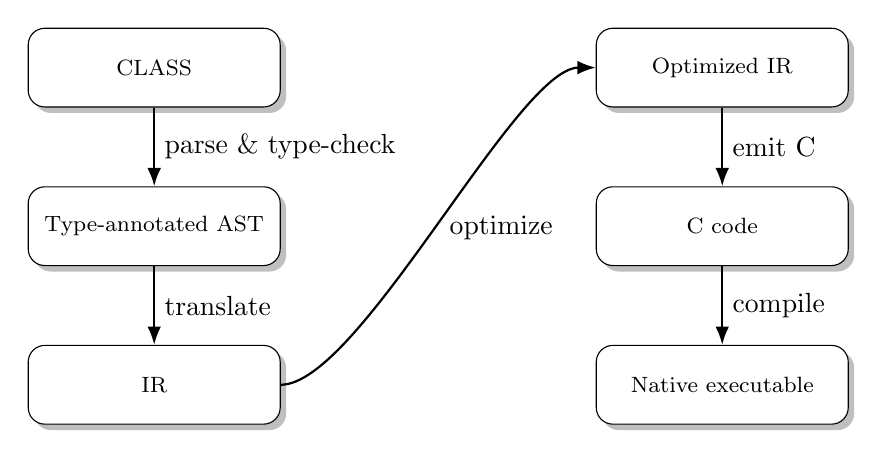
\begin{tikzpicture}[
  box/.style={
    draw, rounded corners=6pt, minimum width=32mm, minimum height=10mm,
    align=center, font=\footnotesize, fill=white, drop shadow
  },
  arr/.style={-Latex, line width=0.8pt},
  node distance=10mm and 20mm
]

% Left column (top to bottom)
\node[box] (class) {CLASS};
\node[box, below=of class] (parser) {Type-annotated AST};
\node[box, below=of parser] (ir) {IR};

% Right column (top to bottom)
\node[box, right=40mm of class] (opt) {Optimized IR};
\node[box, below=of opt] (cgen) {C code};
\node[box, below=of cgen] (native) {Native executable};

% Arrows (left column downward)
\draw[arr] (class) -- node[right]{parse \& type-check} (parser);
\draw[arr] (parser) -- node[right]{translate} (ir);

% Arrows (connecting columns)
\draw[arr] (ir.east) .. controls +(10mm,0) and +(-10mm,0) .. node[above, xshift=8mm, yshift=-3mm]{optimize} (opt.west);

% Arrows (right column downward)

\draw[arr] (opt) -- node[right]{emit C} (cgen);
\draw[arr] (cgen) -- node[right]{compile} (native);

\end{tikzpicture}%
}
\end{frame}

\begin{frame}{The Intermediate Representation (IR)}
\begin{itemize}
  \item \textbf{Purpose:} Bridge between high-level CLASS semantics and low-level C code.
  \item Simplified code generation and optimization.
  \item Sequential execution model inspired by the \textit{Linear Session Abstract Machine (SAM)}. \begin{itemize}
    \item Deterministic, continuation-based control flow.
    \item Buffered communication via data sections.
  \end{itemize}
\end{itemize}
\end{frame}

% \begin{frame}{IR Program Structure}
% \centering
% \begin{tikzpicture}[
%   node distance=7mm and 8mm,
%   every node/.style={font=\footnotesize, align=center},
%   box/.style={
%     draw, rounded corners=4pt, fill=white,
%     minimum width=30mm, minimum height=8mm
%   },
%   arr/.style={-Latex, line width=0.7pt}
% ]

% % Root
% \node[box] (program) {IR Program};

% % Processes
% \node[box, below=of program, xshift=-20mm] (proc1) {Process 1};
% \node[box, below=of program, xshift=20mm] (proc2) {Process n};
% \node at ($(proc1)!0.5!(proc2)$) [below=2mm,font=\scriptsize] {...};

% % Composition arrows
% \draw[arr] (program.south) -- (proc1.north);
% \draw[arr] (program.south) -- (proc2.north);

% % Structure of a process (left)
% \node[box, below=8mm of proc1, xshift=-17mm] (header) {Header};
% \node[box, below=8mm of proc1, xshift=17mm] (body) {Body};

% \draw[arr] (proc1.south) -- (header.north);
% \draw[arr] (proc1.south) -- (body.north);

% % Body details
% \node[box, below=8mm of body, xshift=-20mm] (block1) {Block 1};
% \node[box, below=8mm of body, xshift=20mm] (block2) {Block m};
% \node at ($(block1)!0.5!(block2)$) [below=2mm,font=\scriptsize] {...};
% \draw[arr] (body.south) -- (block1.north);
% \draw[arr] (body.south) -- (block2.north);

% \end{tikzpicture}
% \end{frame}

\note{
  - O modelo de execução da IR, tal como na LSAM, é sequencial e determinístico, com controlo baseado em continuações e comunicação buffered.

  - O estado de execução é descrito por um ambiente $E$, uma espécie de stack-frame alocada no heap, uma pilha de tarefas $T$, pontos de execução a serem retomados no futuro, e um contador de programa.

  - Tal como stack frames contém o estado necessário para executar funções em linguagens como C, ambientes contêm o estado necessário para executar processos. Ao contrário de funções em C, que têm apenas um local para onde retornam, processos podem ser suspensos e retornar várias vezes para diferentes locais.

  - Então, para gerir a memória dos ambientes, estes guardam um contador de pontos de saída, que essencialmente representa o número de traços de execução não concluídos que dependem deste ambiente. Quando chegar a zero, é a memória associada ao ambiente pode ser dealocada.
  
  - Em vez de apenas um endereço de retorno, ambientes guardam várias continuações, que modelam as sessões: guardam um endereço de memória para onde devem ser escritos dados enviados, e um endereço de programa para onde a execução deve saltar quando a sessão terminar our for suspensa.

  - Finalmente, as secções de dados são buffers onde os valores comunicados são realmente guardado, permitindo comunicação assíncrona.
}

\begin{frame}{IR Execution Model}
\begin{itemize}
  \item Execution state: $\langle E, C \rangle$
  \begin{itemize}
    \item $E$ --- Environment (similar to a heap-allocated stack frame)
    \item $C$ --- Program counter (next instruction)
  \end{itemize}
  \item An environment contains the state of:
  \begin{itemize}
    \item Continuations: return addresses/writing locations for sessions
    \item Data sections: buffers holding communicated values
  \end{itemize}
\end{itemize}
\begin{figure}
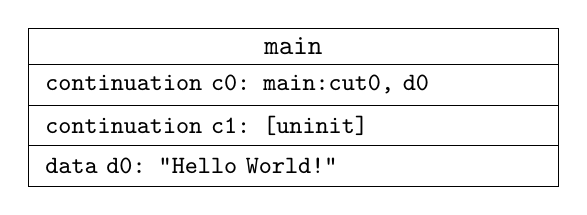
\begin{tikzpicture}
\node[font=\ttfamily] (main title) {main};
\node[row, below=0pt of main title] (main c0) {continuation c0: main:cut0, d0};
\node[row, below=0pt of main c0] (main c1) {continuation c1: [uninit]};
\node[row, below=0pt of main c1] (main d0) {data d0: "Hello World!"};
\node[draw, inner sep=0pt, fit=(main title) (main d0)] (main box) {};
\end{tikzpicture}
\caption{Environment for some process \texttt{main}}
\end{figure}
\end{frame}


\begin{frame}[fragile]{IR Example Program}
\vspace{-7mm}
\begin{lstlisting}[language=CLASS]
proc main() {
  cut { let x 1 |\textbar|x: colint|\textbar| print(x); () }
};;
\end{lstlisting}
\begin{lstlisting}[language=IR]
main:
  continuations: c0
  data d0: <[int]>
entry:
  initContinuation(c0, cut0, d0)
  writeExpression(c0, 1)
  finish(c0)
cut0:
  print(move(d0, int))
  popTask()
\end{lstlisting}
\end{frame}

\begin{frame}[fragile]{Example Execution (1/5)}
\vspace{-3mm}
\begin{lstlisting}[language=IR]
main:
  continuations: c0
  data d0: <[int]>
entry:
  initContinuation(c0, cut0, d0) // <<<<<<<<<<
  writeExpression(c0, 1)
  finish(c0)
cut0:
  print(move(d0, int))
  popTask()
\end{lstlisting}
\begin{center}
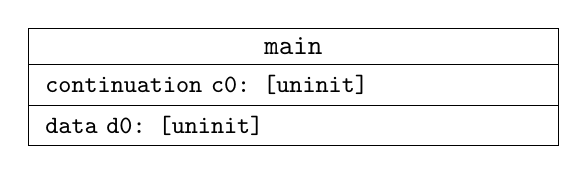
\begin{tikzpicture}
\node[font=\ttfamily] (main title) {main};
\node[row, below=0pt of main title] (main c0) {continuation c0: [uninit]};
\node[row, below=0pt of main c0] (main d0) {data d0: [uninit]};
\node[draw, inner sep=0pt, fit=(main title) (main d0)] (main box) {};
\end{tikzpicture}
\end{center}
\end{frame}

\begin{frame}[fragile]{Example Execution (2/5)}
\vspace{-3mm}
\begin{lstlisting}[language=IR]
main:
  continuations: c0
  data d0: <[int]>
entry:
  initContinuation(c0, cut0, d0)
  writeExpression(c0, 1) // <<<<<<<<<<
  finish(c0)
cut0:
  print(move(d0, int))
  popTask()
\end{lstlisting}
\begin{center}
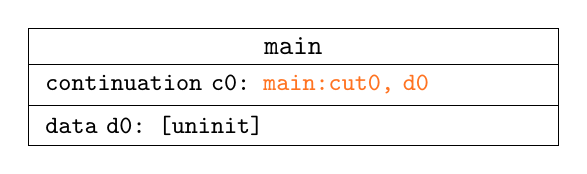
\begin{tikzpicture}
\node[font=\ttfamily] (main title) {main};
\node[row, below=0pt of main title] (main c0) {continuation c0: \changed{main:cut0, d0}};
\node[row, below=0pt of main c0] (main d0) {data d0: [uninit]};
\node[draw, inner sep=0pt, fit=(main title) (main d0)] (main box) {};
\end{tikzpicture}
\end{center}
\end{frame}

\begin{frame}[fragile]{Example Execution (3/5)}
\vspace{-3mm}
\begin{lstlisting}[language=IR]
main:
  continuations: c0
  data d0: <[int]>
entry:
  initContinuation(c0, cut0, d0)
  writeExpression(c0, 1)
  finish(c0) // <<<<<<<<<<
cut0:
  print(move(d0, int))
  popTask()
\end{lstlisting}
\begin{center}
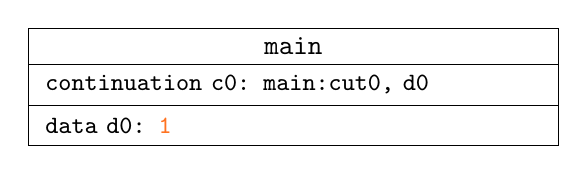
\begin{tikzpicture}
\node[font=\ttfamily] (main title) {main};
\node[row, below=0pt of main title] (main c0) {continuation c0: main:cut0, d0};
\node[row, below=0pt of main c0] (main d0) {data d0: \changed{1}};
\node[draw, inner sep=0pt, fit=(main title) (main d0)] (main box) {};
\end{tikzpicture}
\end{center}
\end{frame}

\begin{frame}[fragile]{Example Execution (4/5)}
\vspace{-3mm}
\begin{lstlisting}[language=IR]
main:
  continuations: c0
  data d0: <[int]>
entry:
  initContinuation(c0, cut0, d0)
  writeExpression(c0, 1)
  finish(c0)
cut0:
  print(move(d0, int)) // <<<<<<<<<<
  popTask()
\end{lstlisting}
\begin{center}
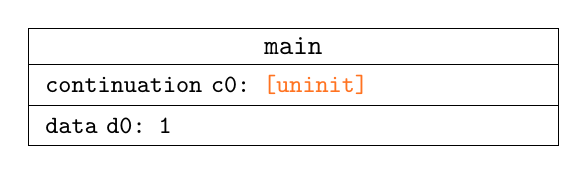
\begin{tikzpicture}
\node[font=\ttfamily] (main title) {main};
\node[row, below=0pt of main title] (main c0) {continuation c0: \changed{[uninit]}};
\node[row, below=0pt of main c0] (main d0) {data d0: 1};
\node[draw, inner sep=0pt, fit=(main title) (main d0)] (main box) {};
\end{tikzpicture}
\end{center}
\end{frame}

\begin{frame}[fragile]{Example Execution (5/5)}
\vspace{-3mm}
\begin{lstlisting}[language=IR]
main:
  continuations: c0
  data d0: <[int]>
entry:
  initContinuation(c0, cut0, d0)
  writeExpression(c0, 1)
  finish(c0)
cut0:
  print(move(d0, int))
  popTask() // <<<<<<<<<<
\end{lstlisting}
\begin{center}
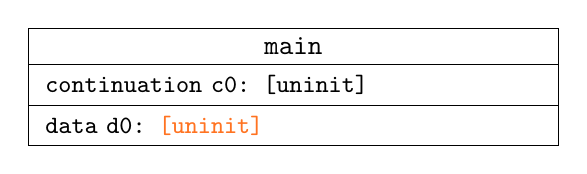
\begin{tikzpicture}
\node[font=\ttfamily] (main title) {main};
\node[row, below=0pt of main title] (main c0) {continuation c0: [uninit]};
\node[row, below=0pt of main c0] (main d0) {data d0: \changed{[uninit]}};
\node[draw, inner sep=0pt, fit=(main title) (main d0)] (main box) {};
\end{tikzpicture}
\end{center}
\end{frame}

\begin{frame}{Optimizing the Compiled Programs}
\begin{itemize}
  \item Leverage type properties to more efficiently represent data. \begin{itemize}
    \item Allows tuples to be stored contiguously, avoiding indirections. 
    \item Compute exponential types once instead of once per usage.
  \end{itemize}
  \item Tail call optimization.
  \item IR program flow/data analysis, and simplifications based on known values.
\end{itemize}
\end{frame}

\begin{frame}[fragile]{Example Compilation: Optimization (1/2)}
\begin{lstlisting}[language=IR]
main:
  continuations: c0
  data d0: <[int]>
entry:
  initContinuation(c0, cut0, d0)
  writeExpression(c0, 1) // known write to d0
  finish(c0) // known jump to cut0
cut0:
  print(move(d0, int))
  popTask()
\end{lstlisting}
\end{frame}

\begin{frame}[fragile]{Example Compilation: Optimization (2/2)}
\begin{lstlisting}[language=IR]
main:
  data d0: <[int]>
entry:
  writeExpression(d0, 1)
  print(move(d0, int))
  popTask()
\end{lstlisting}
\end{frame}

\begin{frame}[fragile]{Example Compilation: Emitting C}
\vspace{-3mm}
\begin{itemize}
  \item Entire IR program compiled into one \texttt{executor()} C function
  \item Instructions operate on the current environment
  \item Address of current environment stored on a register
  \item Environments are heap-allocated buffers with known layouts
  \item Continuations implemented using GCC's \texttt{computed goto}
\end{itemize}
\begin{lstlisting}[language=C]
main_entry:
  // writeExpression(d0, 1)
  *(int*)(env + 0) = 1;
  // print(move(d0, int))
  printf("%d", *(int*)(env + 0));
  // popTask()
  free(env);
\end{lstlisting}
\end{frame}

\section{Results and Conclusion}

\begin{frame}{Results: Implementation and Validation}
\begin{itemize}
  \item Compiler implemented in Java within the existing CLASS/SAM codebase.
  \item Fully covers CLASS, including affine sessions, shared state and polymorphism.
  \item Over \textbf{180 unit tests} written in CLASS verifying semantics and code generation for each language construct.
  \item Test suite also includes complex examples (e.g. prime sieve, game of life), covering use cases encountered in real-world applications.
\end{itemize}
\end{frame}

\begin{frame}{Results: Sieve Benchmarks}
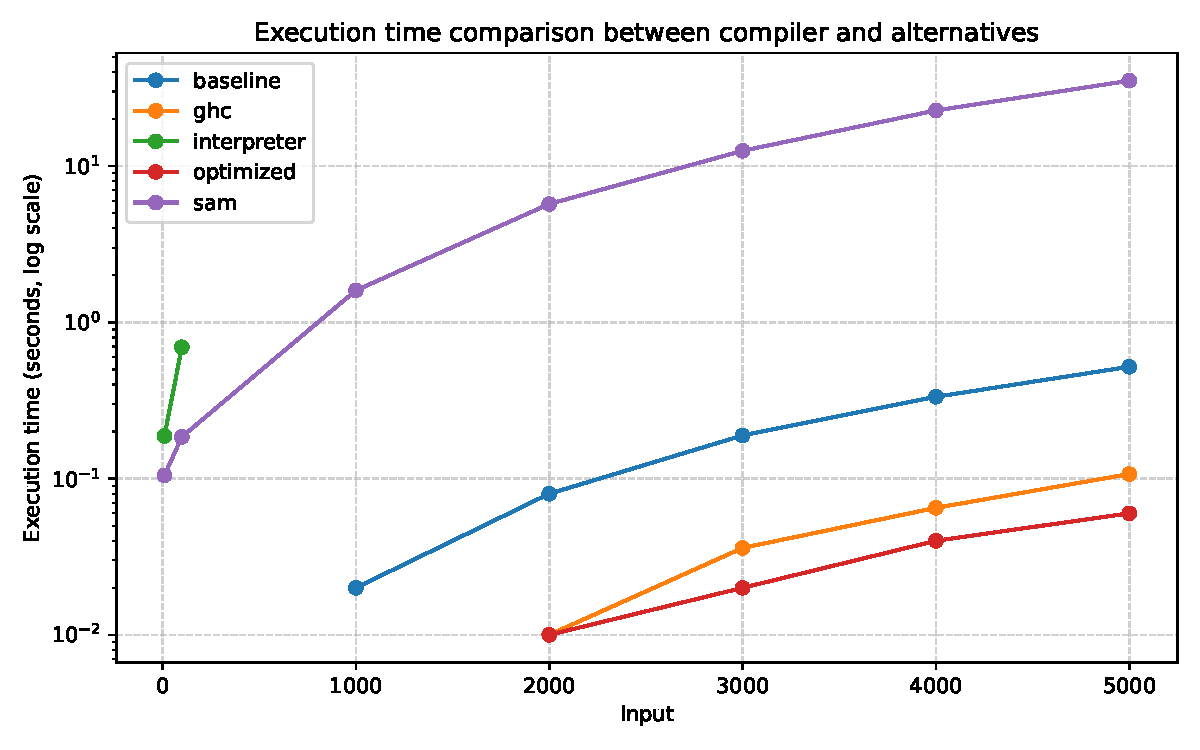
\includegraphics[width=\linewidth]{Images/execution_time_sieve_compiler_vs_alternatives.pdf}
\end{frame}

\begin{frame}{Future Work}
\begin{itemize}
  \item \textbf{Lower-Level Code Generation}
  \begin{itemize}
    \item Target LLVM IR or assembly.
    \item Store frequently accessed data in CPU registers.
  \end{itemize}

  \item \textbf{Standard Library}
  \begin{itemize}
    \item Provide native implementations of data structures.
  \end{itemize}

  \item \textbf{Further IR Optimizations}
  \begin{itemize}
    \item Remove redundant data moves and copies.
    \item Reuse data sections to reduce memory footprint.
  \end{itemize}

  \item \textbf{Formal Verification}
  \begin{itemize}
    \item Develop a proof of correctness for the compilation scheme.
    \item Base the proof on the verified SAM execution model.
  \end{itemize}
\end{itemize}
\end{frame}

\begin{frame}{}
  \begin{center}
    \huge Thank you!
  \end{center}
\end{frame}

\begin{frame}[shrink=20]
  \bibliography{./Bibliography}
\end{frame}

\begin{frame}{Results: Sieve Benchmarks}
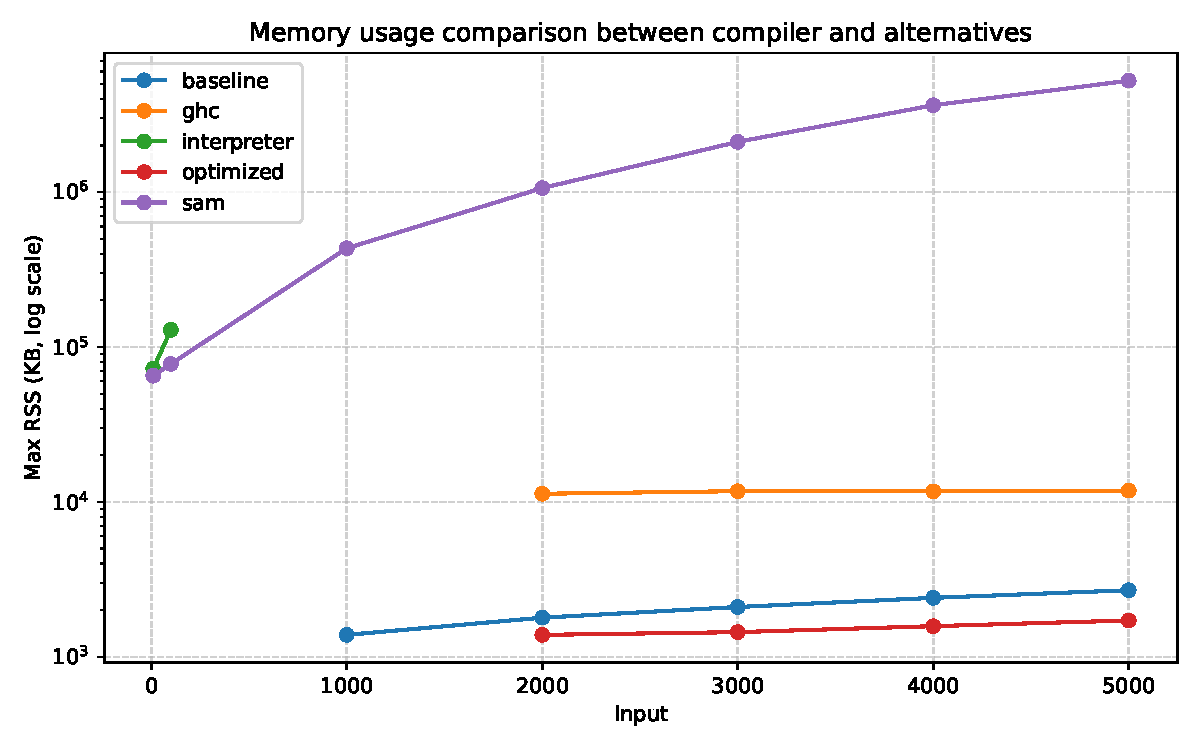
\includegraphics[width=\linewidth]{Images/memory_usage_sieve_compiler_vs_alternatives.pdf}
\end{frame}

\begin{frame}{Results: Game of Life Benchmarks}
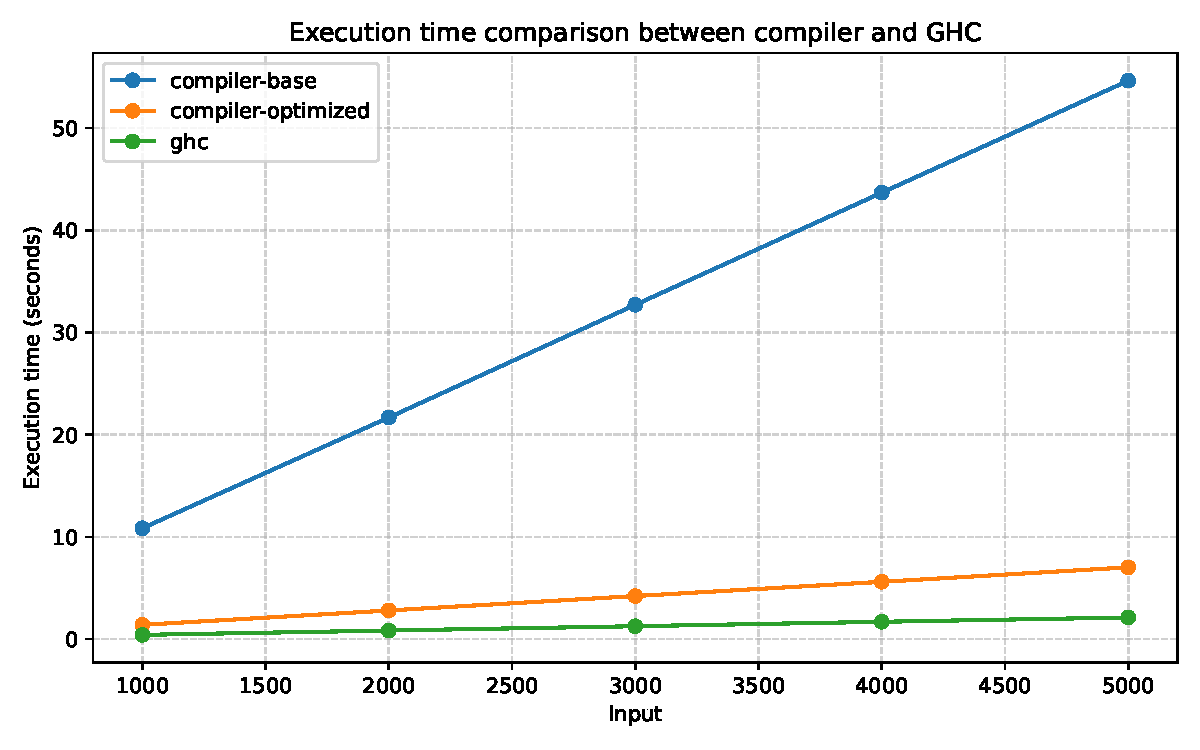
\includegraphics[width=\linewidth]{Images/execution_time_gol_compiler_vs_ghc.pdf}
\end{frame}

\begin{frame}{Results: Game of Life Benchmarks}
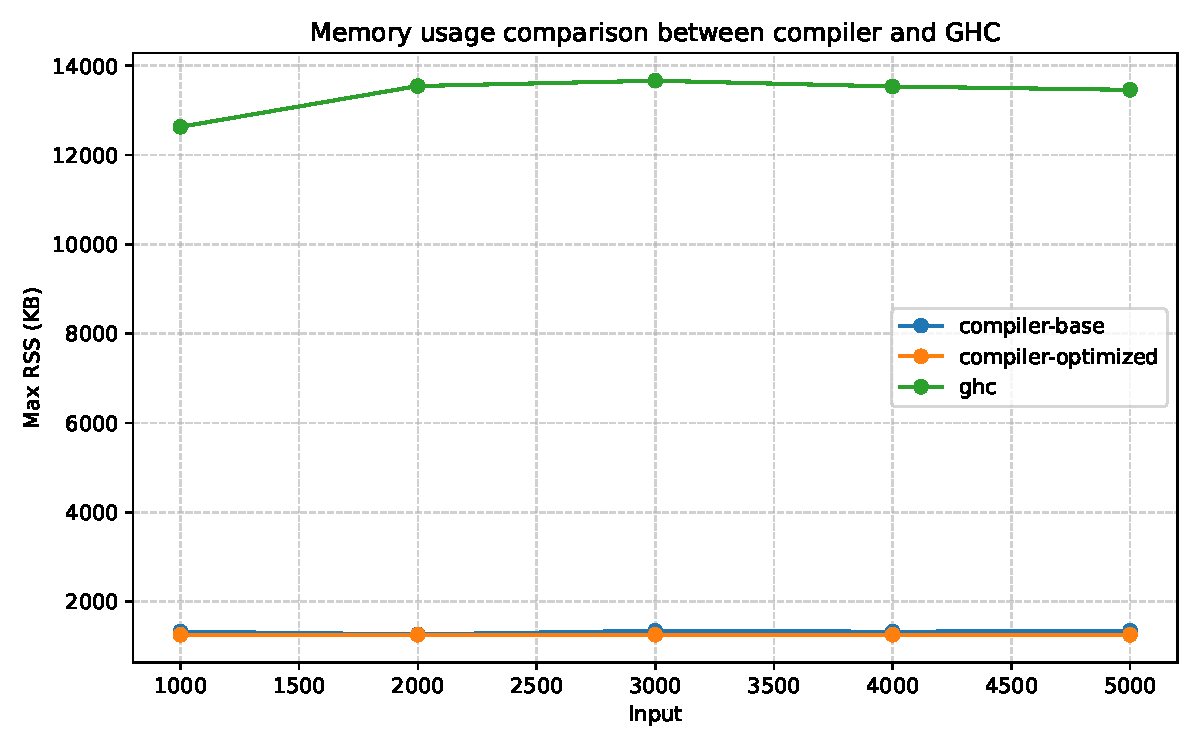
\includegraphics[width=\linewidth]{Images/memory_usage_gol_compiler_vs_ghc.pdf}
\end{frame}

\end{document}
